\documentclass[a4paper,12pt]{article}

% don't forget the document class, generally : \documentclass[a4paper,12pt]{article}

\usepackage[utf8]{inputenc}
\usepackage[french]{babel}
\usepackage{graphicx}
\usepackage{gensymb}
\usepackage{amsmath}
\usepackage{float}
\usepackage{scrextend}
\usepackage{caption} 
\usepackage{siunitx}
\usepackage{enumitem}
\usepackage{amsthm}
\usepackage{fancyhdr}
\usepackage{amssymb}
\usepackage{wrapfig}
\usepackage{geometry}
\usepackage{standalone}
\usepackage{import}
\usepackage[usenames, dvipsnames]{color}

 \usepackage{biblatex} % manages bibliography and references
\addbibresource{sample.bib}


\geometry{hmargin=1in, vmargin=1in}

 \newenvironment{absolutelynopagebreak}
 {\par\nobreak\vfil\penalty0\vfilneg
 \vtop\bgroup}
 {\par\xdef\tpd{\the\prevdepth}\egroup
 \prevdepth=\tpd}
 
 \pagestyle{fancy}                        
\fancyhf{}                               
\fancyhf[HL]{Application des maths}                
\fancyhf[HR]{Géométrie euclidienne}             
\fancyhf[FC]{\thepage/\pageref{Lastpage}}
 
\newtheorem{definition}{Définition}[section]
\newtheorem{theorem}{Théorème}
\newtheorem{corollary}{Corollaire}[theorem]
\newtheorem{lemma}[theorem]{Lemme}
\newtheorem*{hyp}{Hypothèse}
\newtheorem*{concl}{Conclusion}
\newtheorem*{remark}{Remarque}

\captionsetup{format=default,labelformat=simple,labelsep=colon,
justification=justified,font={sf,small},labelfont=bf,
textfont=default} 



\begin{document}

\pagebreak
\subsection{Cosinus de la différence de deux angles}
\begin{theorem}
Le cosinus de la différence de deux angles est égal à la somme du produit de leurs sinus et du produit de leurs cosinus.
\begin{equation}
    cos(\beta-\alpha) = cos \alpha \cdot cos \beta + sin \alpha \cdot sin \beta
\end{equation}
\end{theorem}
\begin{figure}[H]
    \centering
    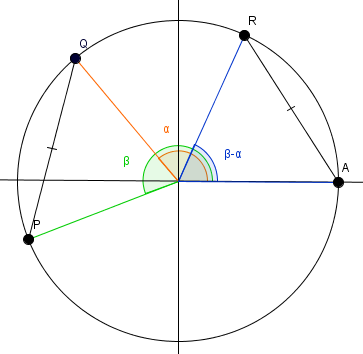
\includegraphics[scale=0.8]{schema/diff.PNG}
\end{figure}

\begin{proof}
Nous considérons le cercle trigonométrique suivant, dans lequel nous avons représenté l'angle $\beta-\alpha$, que nous avons reporté sur l'axe du cosinus (grâce à l'axiome de report). Ainsi, en reliant les points QP et les points AR, nous obtenons deux triangles ayant un angle isométrique compris entre deux côtés isométriques. Ce qui signifie que les triangles $\Delta ARO$ et $\Delta PQO$ sont isométriques (axiome III). Donc, on peut écrire que:
\begin{equation}
    ||\vec{PQ}|| \equiv ||\vec{AR}||
\end{equation}

On connait aussi les coordonnées des quatre points P, Q, A et R, qui sont:
\begin{equation}
\begin{split}
   & P = (cos \beta, sin \beta)\\
   & Q = (cos \alpha, sin \alpha)\\
   & A = (1, 0)\\
   & R = (cos (\beta-\alpha), sin (\beta-\alpha))
\end{split}
\end{equation}

Donc, on peut décrire les vecteurs $\vec{PQ}$ et $\vec{AR}$ de la manière suivante:

\begin{equation}
\begin{split}
 & \vec{PQ} = \binom{cos\alpha-cos\beta}{sin\alpha-sin\beta} \rightarrow ||\vec{PQ}|| = \sqrt{(cos\alpha-cos\beta)^2 + (sin\alpha-sin\beta)^2}\\
 & \vec{AR} = \binom{cos(\beta-\alpha)-1}{sin(\beta-\alpha)} \rightarrow ||\vec{AR}|| = \sqrt{(cos(\beta-\alpha)-1)^2 + (sin(\beta-\alpha)^2}
\end{split}
\end{equation}

Finalement, comme $||\vec{PQ}||$ et $||\vec{AR}||$ sont équivalents, on peut écrire l'égalité suivante:
\begin{equation}
(cos(\beta-\alpha)-1)^2 + (sin(\beta-\alpha)^2 = (cos\alpha-cos\beta)^2 + (sin\alpha-sin\beta)^2
\end{equation}
Ce qui développé donne:
\begin{equation}
2-2cos(\beta-\alpha) = 2-2(cos \alpha \cdot cos \beta + sin \alpha \cdot sin \beta)
\end{equation}
Nous avons donc démontré la formule du cosinus de la différence de deux angles:
\begin{equation*}
    cos(\beta-\alpha) = cos \alpha \cdot cos \beta + sin \alpha \cdot sin \beta
\end{equation*}
\end{proof}

\end{document}